\section{Geom  Class Reference}
\label{class_Geom}\index{Geom@{Geom}}
Geometric models and collision detection methods. 


{\tt \#include $<$geom.h$>$}

Inheritance diagram for Geom::\begin{figure}[H]
\begin{center}
\leavevmode
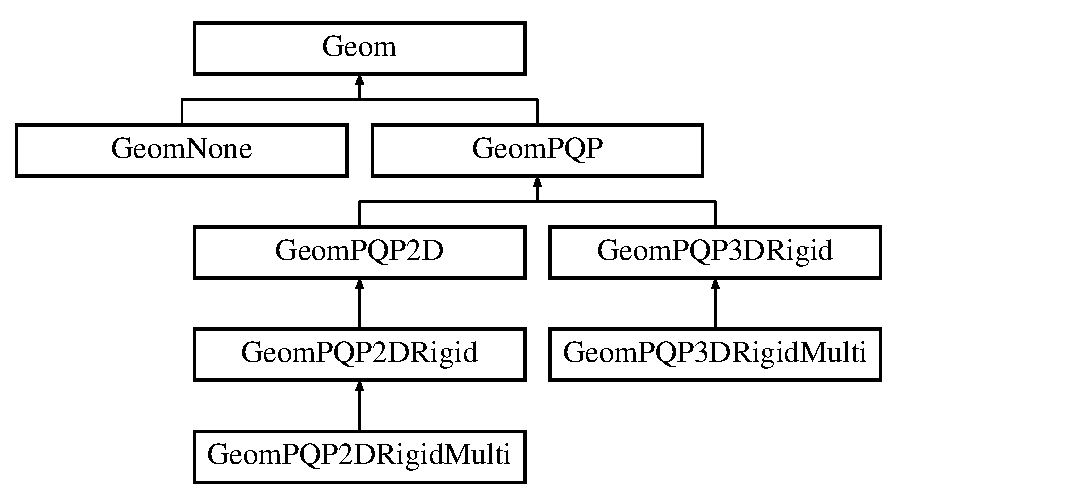
\includegraphics[height=5cm]{class_Geom}
\end{center}
\end{figure}
\subsection*{Public Methods}
\begin{CompactItemize}
\item 
{\bf Geom} (string path)
\begin{CompactList}\small\item\em Empty constructor in base class.\item\end{CompactList}\item 
virtual {\bf $\sim$Geom} ()
\begin{CompactList}\small\item\em Empty destructor.\item\end{CompactList}\item 
virtual bool {\bf Collision\-Free} (const {\bf MSLVector} \&q)=0
\begin{CompactList}\small\item\em Return true if the robot(s) and obstacles are not in collision.\item\end{CompactList}\item 
virtual double {\bf Distance\-Comp} (const {\bf MSLVector} \&q)=0
\begin{CompactList}\small\item\em Compute the distance of the closest point on the robot to the obstacle region.\item\end{CompactList}\item 
virtual {\bf MSLVector} {\bf Configuration\-Difference} (const {\bf MSLVector} \&q1, const {\bf MSLVector} \&q2)
\begin{CompactList}\small\item\em Compute a {\bf MSLVector} {\rm (p.\,\pageref{class_MSLVector})} based on q2-q1. In R$^\wedge$n, the configurations are simply subtracted to make the {\bf MSLVector} {\rm (p.\,\pageref{class_MSLVector})}. This method exists to make things work correctly for other configuration-space topologies.\item\end{CompactList}\end{CompactItemize}
\subsection*{Public Attributes}
\begin{CompactItemize}
\item 
int {\bf Num\-Bodies}
\begin{CompactList}\small\item\em The number of rigid bodies in the geometry model.\item\end{CompactList}\item 
int {\bf Geom\-Dim}
\begin{CompactList}\small\item\em The dimension of the world geometry: 2 or 3.\item\end{CompactList}\item 
{\bf MSLVector} {\bf Max\-Deviates}
\begin{CompactList}\small\item\em Maximum displacement of geometry with respect to change in each variable.\item\end{CompactList}\end{CompactItemize}
\subsection*{Protected Attributes}
\begin{CompactItemize}
\item 
string {\bf File\-Path}
\end{CompactItemize}


\subsection{Detailed Description}
Geometric models and collision detection methods.

These classes define the geometric representations of all obstacles in the world, and of each part of the robot. The methods allow planning algorithms to determine whether any of the robot parts are in collision with each other or with obstacles in the world.

A configuration vector specifies the positions and orientation of each rigid body. 



\subsection{Constructor \& Destructor Documentation}
\index{Geom@{Geom}!Geom@{Geom}}
\index{Geom@{Geom}!Geom@{Geom}}
\subsubsection{\setlength{\rightskip}{0pt plus 5cm}Geom::Geom (string {\em path})}\label{class_Geom_a0}


Empty constructor in base class.

\index{Geom@{Geom}!~Geom@{$\sim$Geom}}
\index{~Geom@{$\sim$Geom}!Geom@{Geom}}
\subsubsection{\setlength{\rightskip}{0pt plus 5cm}Geom::$\sim$Geom ()\hspace{0.3cm}{\tt  [inline, virtual]}}\label{class_Geom_a1}


Empty destructor.



\subsection{Member Function Documentation}
\index{Geom@{Geom}!CollisionFree@{CollisionFree}}
\index{CollisionFree@{CollisionFree}!Geom@{Geom}}
\subsubsection{\setlength{\rightskip}{0pt plus 5cm}bool Geom::Collision\-Free (const {\bf MSLVector} \& {\em q})\hspace{0.3cm}{\tt  [pure virtual]}}\label{class_Geom_a2}


Return true if the robot(s) and obstacles are not in collision.



Reimplemented in {\bf Geom\-None} {\rm (p.\,\pageref{class_GeomNone_a2})}, {\bf Geom\-PQP} {\rm (p.\,\pageref{class_GeomPQP_a4})}, {\bf Geom\-PQP2DRigid} {\rm (p.\,\pageref{class_GeomPQP2DRigid_a2})}, {\bf Geom\-PQP2DRigid\-Multi} {\rm (p.\,\pageref{class_GeomPQP2DRigidMulti_a2})}, {\bf Geom\-PQP3DRigid} {\rm (p.\,\pageref{class_GeomPQP3DRigid_a2})}, and {\bf Geom\-PQP3DRigid\-Multi} {\rm (p.\,\pageref{class_GeomPQP3DRigidMulti_a2})}.\index{Geom@{Geom}!ConfigurationDifference@{ConfigurationDifference}}
\index{ConfigurationDifference@{ConfigurationDifference}!Geom@{Geom}}
\subsubsection{\setlength{\rightskip}{0pt plus 5cm}{\bf MSLVector} Geom::Configuration\-Difference (const {\bf MSLVector} \& {\em q1}, const {\bf MSLVector} \& {\em q2})\hspace{0.3cm}{\tt  [virtual]}}\label{class_Geom_a4}


Compute a {\bf MSLVector} {\rm (p.\,\pageref{class_MSLVector})} based on q2-q1. In R$^\wedge$n, the configurations are simply subtracted to make the {\bf MSLVector} {\rm (p.\,\pageref{class_MSLVector})}. This method exists to make things work correctly for other configuration-space topologies.



Reimplemented in {\bf Geom\-PQP2DRigid} {\rm (p.\,\pageref{class_GeomPQP2DRigid_a4})}, and {\bf Geom\-PQP3DRigid} {\rm (p.\,\pageref{class_GeomPQP3DRigid_a4})}.\index{Geom@{Geom}!DistanceComp@{DistanceComp}}
\index{DistanceComp@{DistanceComp}!Geom@{Geom}}
\subsubsection{\setlength{\rightskip}{0pt plus 5cm}double Geom::Distance\-Comp (const {\bf MSLVector} \& {\em q})\hspace{0.3cm}{\tt  [pure virtual]}}\label{class_Geom_a3}


Compute the distance of the closest point on the robot to the obstacle region.



Reimplemented in {\bf Geom\-None} {\rm (p.\,\pageref{class_GeomNone_a3})}, {\bf Geom\-PQP} {\rm (p.\,\pageref{class_GeomPQP_a5})}, {\bf Geom\-PQP2DRigid} {\rm (p.\,\pageref{class_GeomPQP2DRigid_a3})}, {\bf Geom\-PQP2DRigid\-Multi} {\rm (p.\,\pageref{class_GeomPQP2DRigidMulti_a3})}, {\bf Geom\-PQP3DRigid} {\rm (p.\,\pageref{class_GeomPQP3DRigid_a3})}, and {\bf Geom\-PQP3DRigid\-Multi} {\rm (p.\,\pageref{class_GeomPQP3DRigidMulti_a3})}.

\subsection{Member Data Documentation}
\index{Geom@{Geom}!FilePath@{FilePath}}
\index{FilePath@{FilePath}!Geom@{Geom}}
\subsubsection{\setlength{\rightskip}{0pt plus 5cm}string Geom::File\-Path\hspace{0.3cm}{\tt  [protected]}}\label{class_Geom_n0}


\index{Geom@{Geom}!GeomDim@{GeomDim}}
\index{GeomDim@{GeomDim}!Geom@{Geom}}
\subsubsection{\setlength{\rightskip}{0pt plus 5cm}int Geom::Geom\-Dim}\label{class_Geom_m1}


The dimension of the world geometry: 2 or 3.

\index{Geom@{Geom}!MaxDeviates@{MaxDeviates}}
\index{MaxDeviates@{MaxDeviates}!Geom@{Geom}}
\subsubsection{\setlength{\rightskip}{0pt plus 5cm}{\bf MSLVector} Geom::Max\-Deviates}\label{class_Geom_m2}


Maximum displacement of geometry with respect to change in each variable.

\index{Geom@{Geom}!NumBodies@{NumBodies}}
\index{NumBodies@{NumBodies}!Geom@{Geom}}
\subsubsection{\setlength{\rightskip}{0pt plus 5cm}int Geom::Num\-Bodies}\label{class_Geom_m0}


The number of rigid bodies in the geometry model.



The documentation for this class was generated from the following file:\begin{CompactItemize}
\item 
{\bf geom.h}\end{CompactItemize}
